\chapter{Introducci\'on}
\label{ch:intro}

La observaci\'on del universo ha intrigado a la humanidad desde 

\section{Rayos c\'osmicos}


	\begin{figure}[ht]
		\begin{center}
		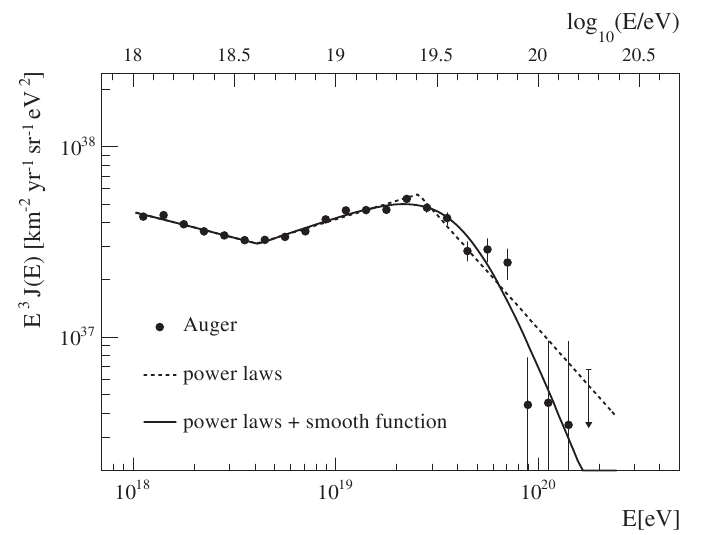
\includegraphics[width=0.75\textwidth]{fig/introduccion/spectrum_withGZK}
		\caption{\label{fig:specGZK} }
		\end{center}
	\end{figure}
	
	\section{Importancia de la detecci\'on de neutrinos c\'osmicos}

	VER EL PROPOSAL DE GRAND!
	
\begin{figure}[ht]
	\begin{center}
	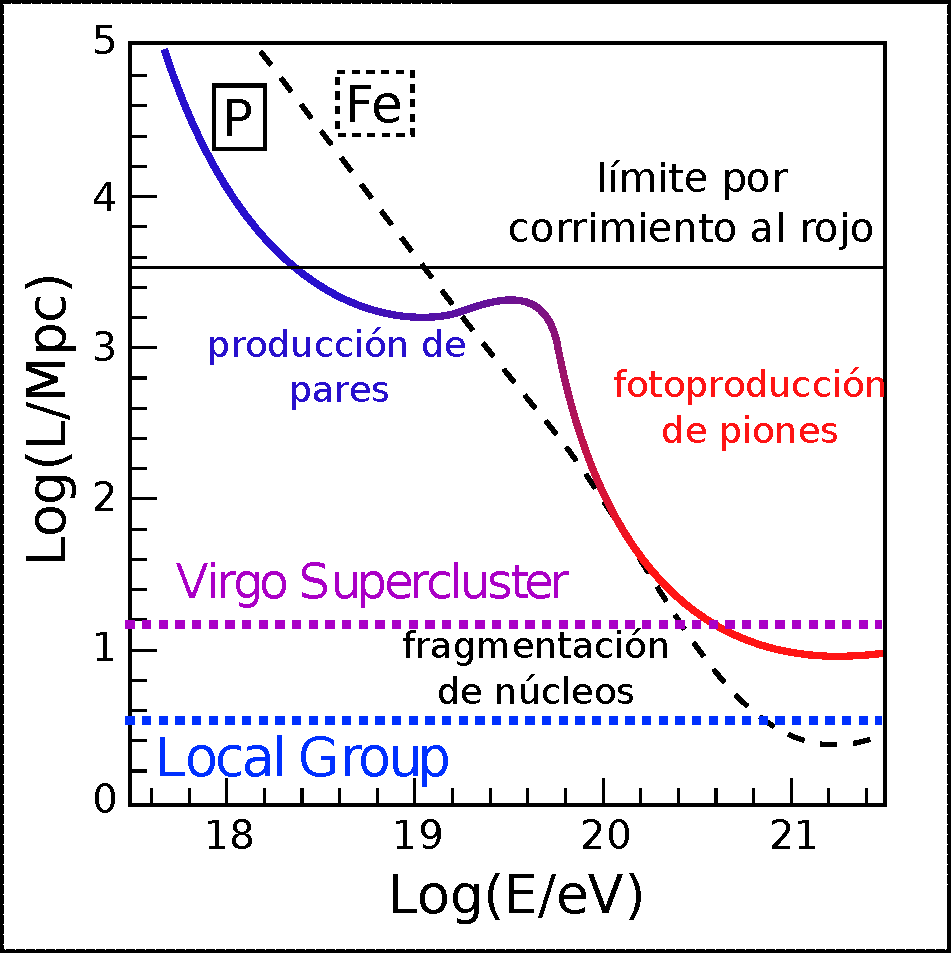
\includegraphics[width=0.75\textwidth]{fig/introduccion/proton_propaga_espanol}
	\caption{\label{fig:protProp} }
	\end{center}
\end{figure}


\begin{figure}[ht]
	\begin{center}
	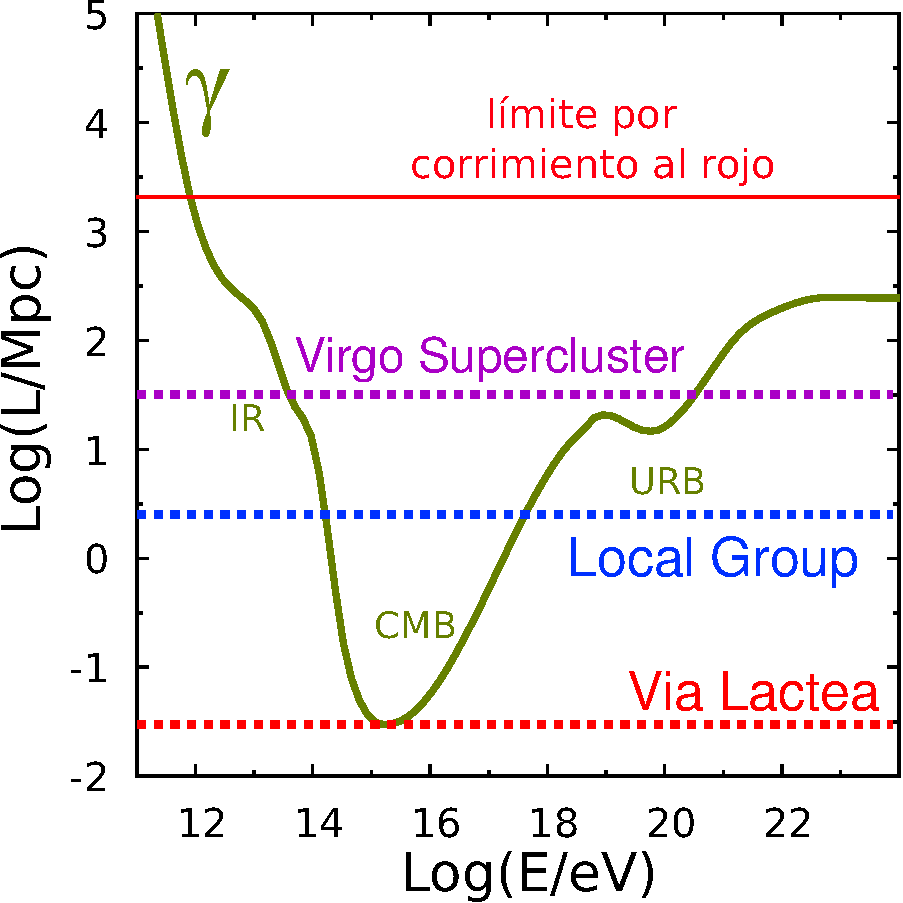
\includegraphics[width=0.75\textwidth]{fig/introduccion/photon_propaga_espanol}
	\caption{\label{fig:photProp} }
	\end{center}
\end{figure}

\section{Posibles fuentes y flujos esperados}

	\subsection{Neutrinos GZK}

	\begin{figure}[ht]
		\begin{center}
		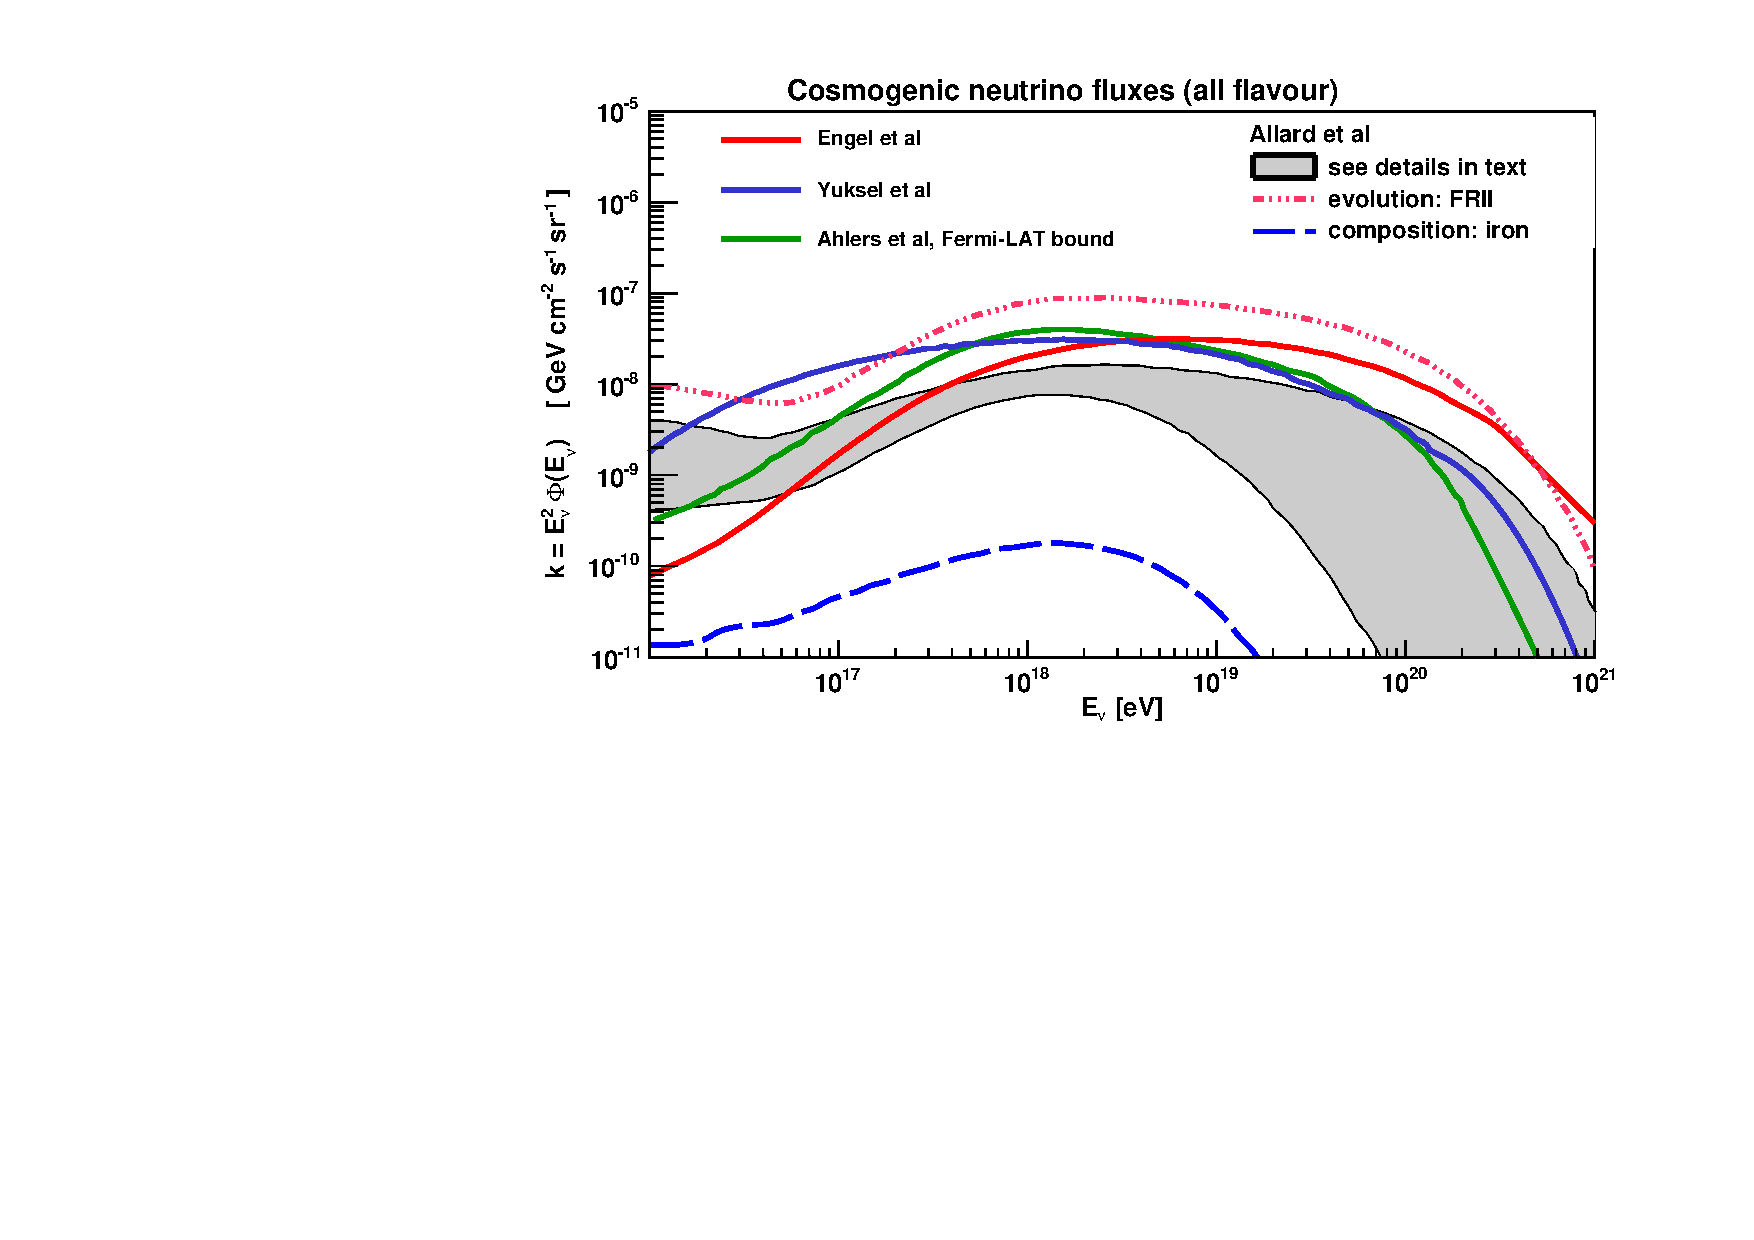
\includegraphics[width=\textwidth]{fig/introduccion/gzk_fluxes}
		\caption{\label{fig:flujosGZK} }
		\end{center}
	\end{figure}
	
	\subsection{AGNs y GRBs}
	
	\begin{figure}[ht]
		\begin{center}
		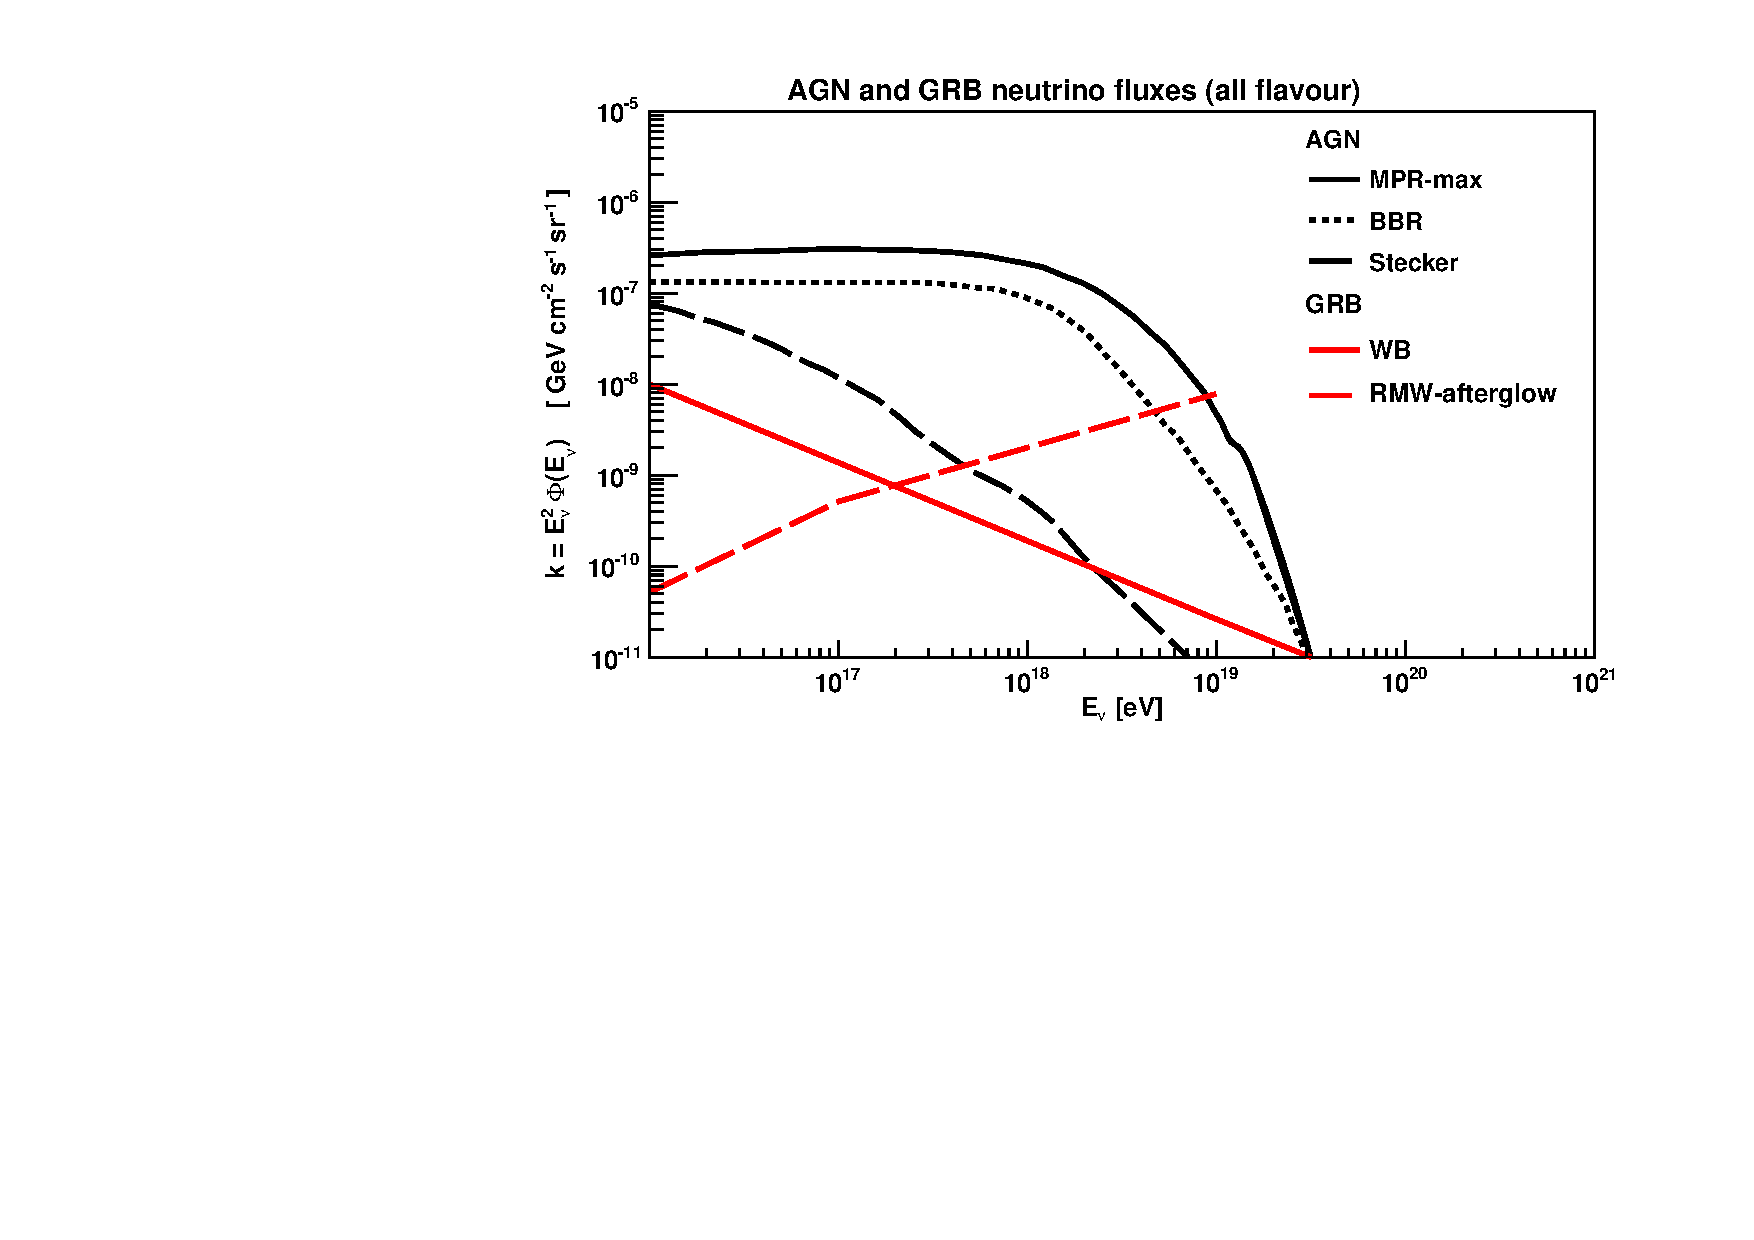
\includegraphics[width=0.75\textwidth]{fig/introduccion/AGN_GRB_nufluxes}
		\caption{\label{fig:flujosAGN} }
		\end{center}
	\end{figure}
	
	\subsection{Fuentes no convencionales}
	
	\begin{figure}[ht]
		\begin{center}
		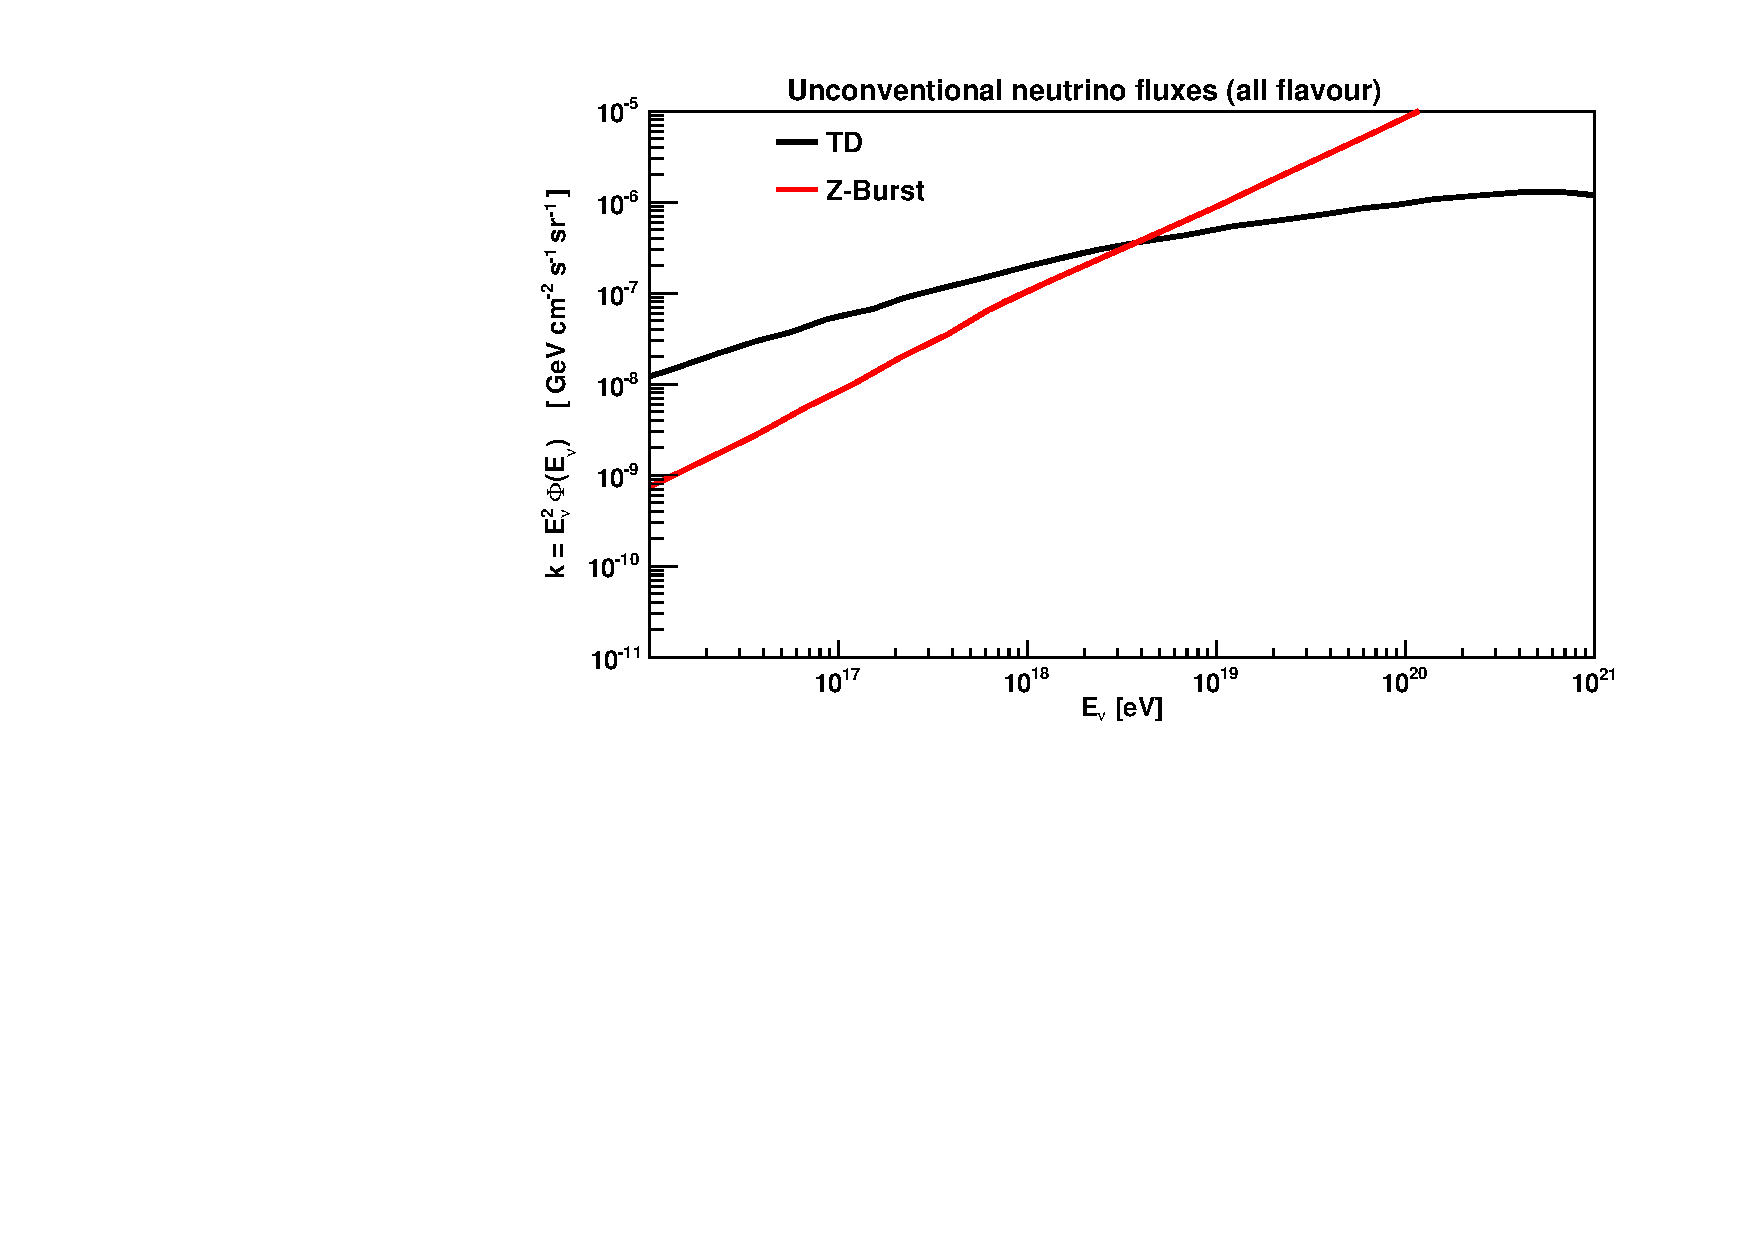
\includegraphics[width=0.75\textwidth]{fig/introduccion/unconventional_nuFluxes}
		\caption{\label{fig:flujosNoConv} }
		\end{center}
	\end{figure}

\section{Búsquedas de neutrinos cósmicos ultra energéticos}

\section{Nacimiento de la astronom\'ia de neutrinos c\'osmicos}

